\documentclass[a4paper,14pt]{extreport}
    \usepackage[left=1.5cm,right=1.5cm,
        top=1.5cm,bottom=2cm,bindingoffset=0cm]{geometry}
    \usepackage{scrextend}
    \usepackage[T1,T2A]{fontenc}
    \usepackage[utf8]{inputenc}
    \usepackage[english,russian,ukrainian]{babel}
    \usepackage{tabularx}
    \linespread{1.5}
    \usepackage{amssymb}
    \usepackage{color}
    \usepackage{amsmath}
    \usepackage{mathrsfs}
    \usepackage{listings}
    \usepackage{graphicx}
    \graphicspath{ {./images/} }
    \usepackage{lipsum}
    \usepackage{xcolor}
    \usepackage{hyperref}
    \usepackage{tcolorbox}
    \usepackage{tikz}
    \usepackage[framemethod=TikZ]{mdframed}
    \usepackage{wrapfig,boxedminipage,lipsum}
    \mdfdefinestyle{MyFrame}{%
    linecolor=blue,outerlinewidth=2pt,roundcorner=20pt,innertopmargin=\baselineskip,innerbottommargin=\baselineskip,innerrightmargin=20pt,innerleftmargin=20pt,backgroundcolor=gray!50!white}
     \usepackage{csvsimple}
     \usepackage{supertabular}
    \usepackage{pdflscape}
    \usepackage{fancyvrb}
    %\usepackage{comment}
    \usepackage{array,tabularx}
    \usepackage{colortbl}

    \usepackage{varwidth}
    \tcbuselibrary{skins}
    \usepackage{fancybox}


    \usepackage{tikz}
    \usepackage[framemethod=TikZ]{mdframed}
    \usepackage{xcolor}
    \usetikzlibrary{calc}
    \makeatletter
    \newlength{\mylength}
    \xdef\CircleFactor{1.1}
    \setlength\mylength{\dimexpr\f@size pt}
    \newsavebox{\mybox}
    \newcommand*\circled[2][draw=blue]{\savebox\mybox{\vbox{\vphantom{WL1/}#1}}\setlength\mylength{\dimexpr\CircleFactor\dimexpr\ht\mybox+\dp\mybox\relax\relax}\tikzset{mystyle/.style={circle,#1,minimum height={\mylength}}}
    \tikz[baseline=(char.base)]
    \node[mystyle] (char) {#2};}
    \makeatother

    \definecolor{ggreen}{rgb}{0.4,1,0}
    \definecolor{rred}{rgb}{1,0.1,0.1}
    \definecolor{amber}{rgb}{1.0, 0.75, 0.0}
    \definecolor{babyblue}{rgb}{0.54, 0.81, 0.94}
    \definecolor{asparagus}{rgb}{0.53, 0.66, 0.42}
    \definecolor{chartreuse}{rgb}{0.5, 1.0, 0.0}
    \definecolor{darkorchid}{rgb}{0.6, 0.2, 0.8}

    \usepackage{float}
    \usepackage{wrapfig}
    \usepackage{framed}
    %for nice Code{
    \lstdefinestyle{customc}{
      belowcaptionskip=1\baselineskip,
      breaklines=true,
      frame=L,
      xleftmargin=\parindent,
      language=C,
      showstringspaces=false,
      basicstyle=\small\ttfamily,
      keywordstyle=\bfseries\color{green!40!black},
      commentstyle=\itshape\color{purple!40!black},
      identifierstyle=\color{blue},
      stringstyle=\color{orange},
    }
    \lstset{escapechar=@,style=customc}
%}


\begin{document}
\pagecolor{white}

\begin{center}
Індивідуальне тестове завдання 2 вар. № 54
\end{center}


\begin{enumerate}
  \item 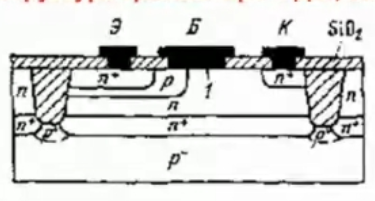
\includegraphics[width=0.4\linewidth]{11.png}
  \item 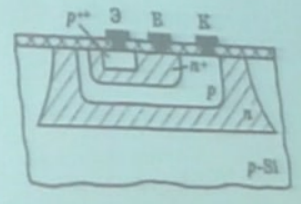
\includegraphics[width=0.4\linewidth]{33.png}
  \item Транзистори середньої та великої потужності працюють в схемах в режимі високих щільностей емітерного струму. При високих рівнях інжекцї зростає базовий струм, тому необхідно враховувати спад напруги вздовж бази. Напруга на емітерному переході являє собою різницю зовнішньої напруги та спад напруги в об'ємі бази. Отже, напруга в центральній частині емітера менша напруги з країв емітера та розподілення струму по площі емітера є неоднорідним, тобто відбувається витіснення струму до периферійної частини емітера. Це означає, що зовнішня частина емітера працює при підвищених щільностях струму, а його зовнішня центральна частина - при понижених. Якщо площу емітера вибрати, виходячи з деякої середньої допустимої щільності струму, то крайові області емітера будуть працювати в умовах перевантаження, тоді як центральна частина буде недовантаженою. Підвищена щільність струму 3 боків емітера призведе до підвищення втрат на поверхневу рекомбінацію і до пониження коефіцієнта передачі струму. Тому в потужних транзисторах краще використовувати вузькі емітери з великим периметром.\par
  Топологія транзистора розробляється так, щоб забезпечити максимальне відношення периметра емітера до його площі. Тим самим вдається значно підвищити активну область транзисторної структури та забезпечити достатньо великий робочий струм без збільшення загальних розмірів всієї структури.
  \item Розширити базовий контакт, додати захисне охоронне кільце або використовувати перше і друге одночасно.
  \begin{figure}[h]
  \item 
        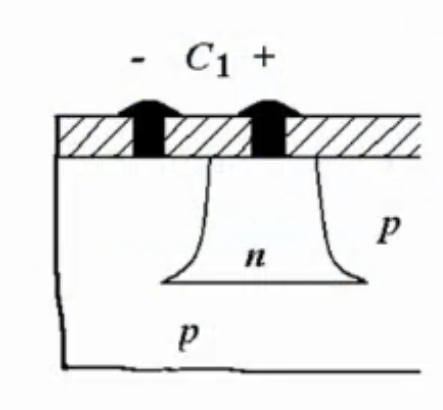
\includegraphics[width=0.4\linewidth]{55.png}
        \caption{конденсатор на основі ізолюючого p-n переходу}
        
        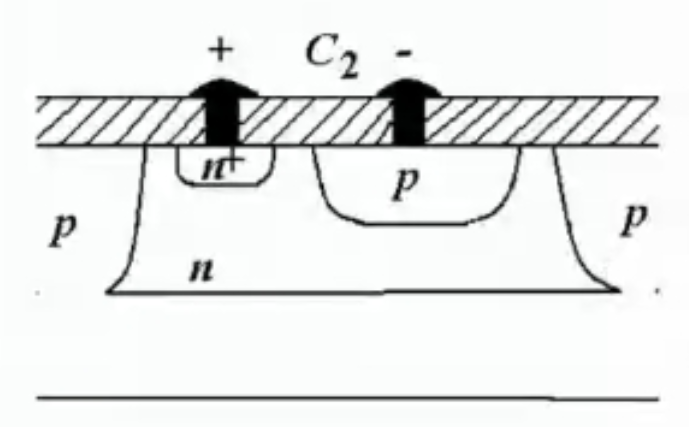
\includegraphics[width=0.4\linewidth]{66.png}
        \caption{конденсатор на основі колекторного переходу}
        
        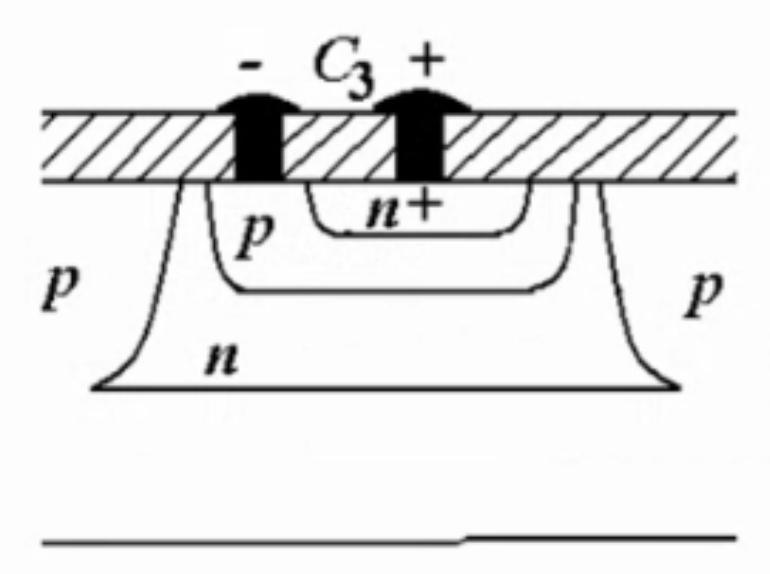
\includegraphics[width=0.4\linewidth]{77.png}
        \caption{конденсатор на основі емітерного переходу}
        
   \end{figure}

  \begin{figure}[h]\item 
        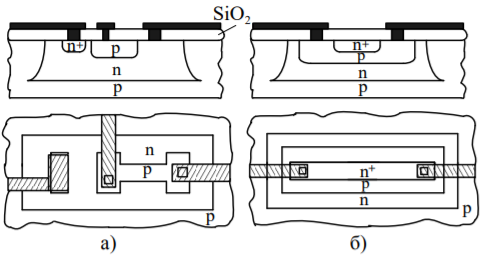
\includegraphics[width=0.4\linewidth]{44.png}
        \caption{Конструкції пінч-резисторив а) на основі базового шару б) на основі колекторної області}
        \label{r1}
        
        При необхідності створення високоомних резисторів з опором більше 60 кОм використовують пінч-резистори (канальні, стислі або закриті). Пінч-резистори можуть створюватися на основі базового або колекторного шарів. На рис. 2.6, а подано конструкцію пінч-резистара на основі базового шару, обмеженого по товщині емітерним шаром $n$ -типу. Резистор являє собою тонкий канал $p$ -типу, в якому використовується донна, слаболегована частина базової області з $R_{s}=2-5$ кОм/$\square$, ізольована зі всіх сторін зворотно змшеним $p-n$ -переходом, оскільки емітерний шар $n$ -типу за межами резистора з'єДнується 3 епітаксіальним $p$ -шаром ізольованої області. Максимальний опір таких резисторів складає $200-300$ кОм при найпростішій смуговій конструкцїї. На рис.\ref{r1} наведено конструкцію пінч-резистора на основі колекторної області, поперечний переріз якого зменшено на глибину базового шару $\left(R_{s}=4-8\right)$ кОм/$\square$. Для отримання якісного омічного контакту використовують дифузійні $n$ -області, що створюються на стадїї емітерної дифузїї. Пінч-резистори мають великий розкид номіналів (до $50 \%)$ через труднощі отримання точних значень товщини донної частини; опір їх сильно залежить від температури внаслідок малого ступеня легування областей, на основі яких вони виконуються.
        \end{figure}
  \item 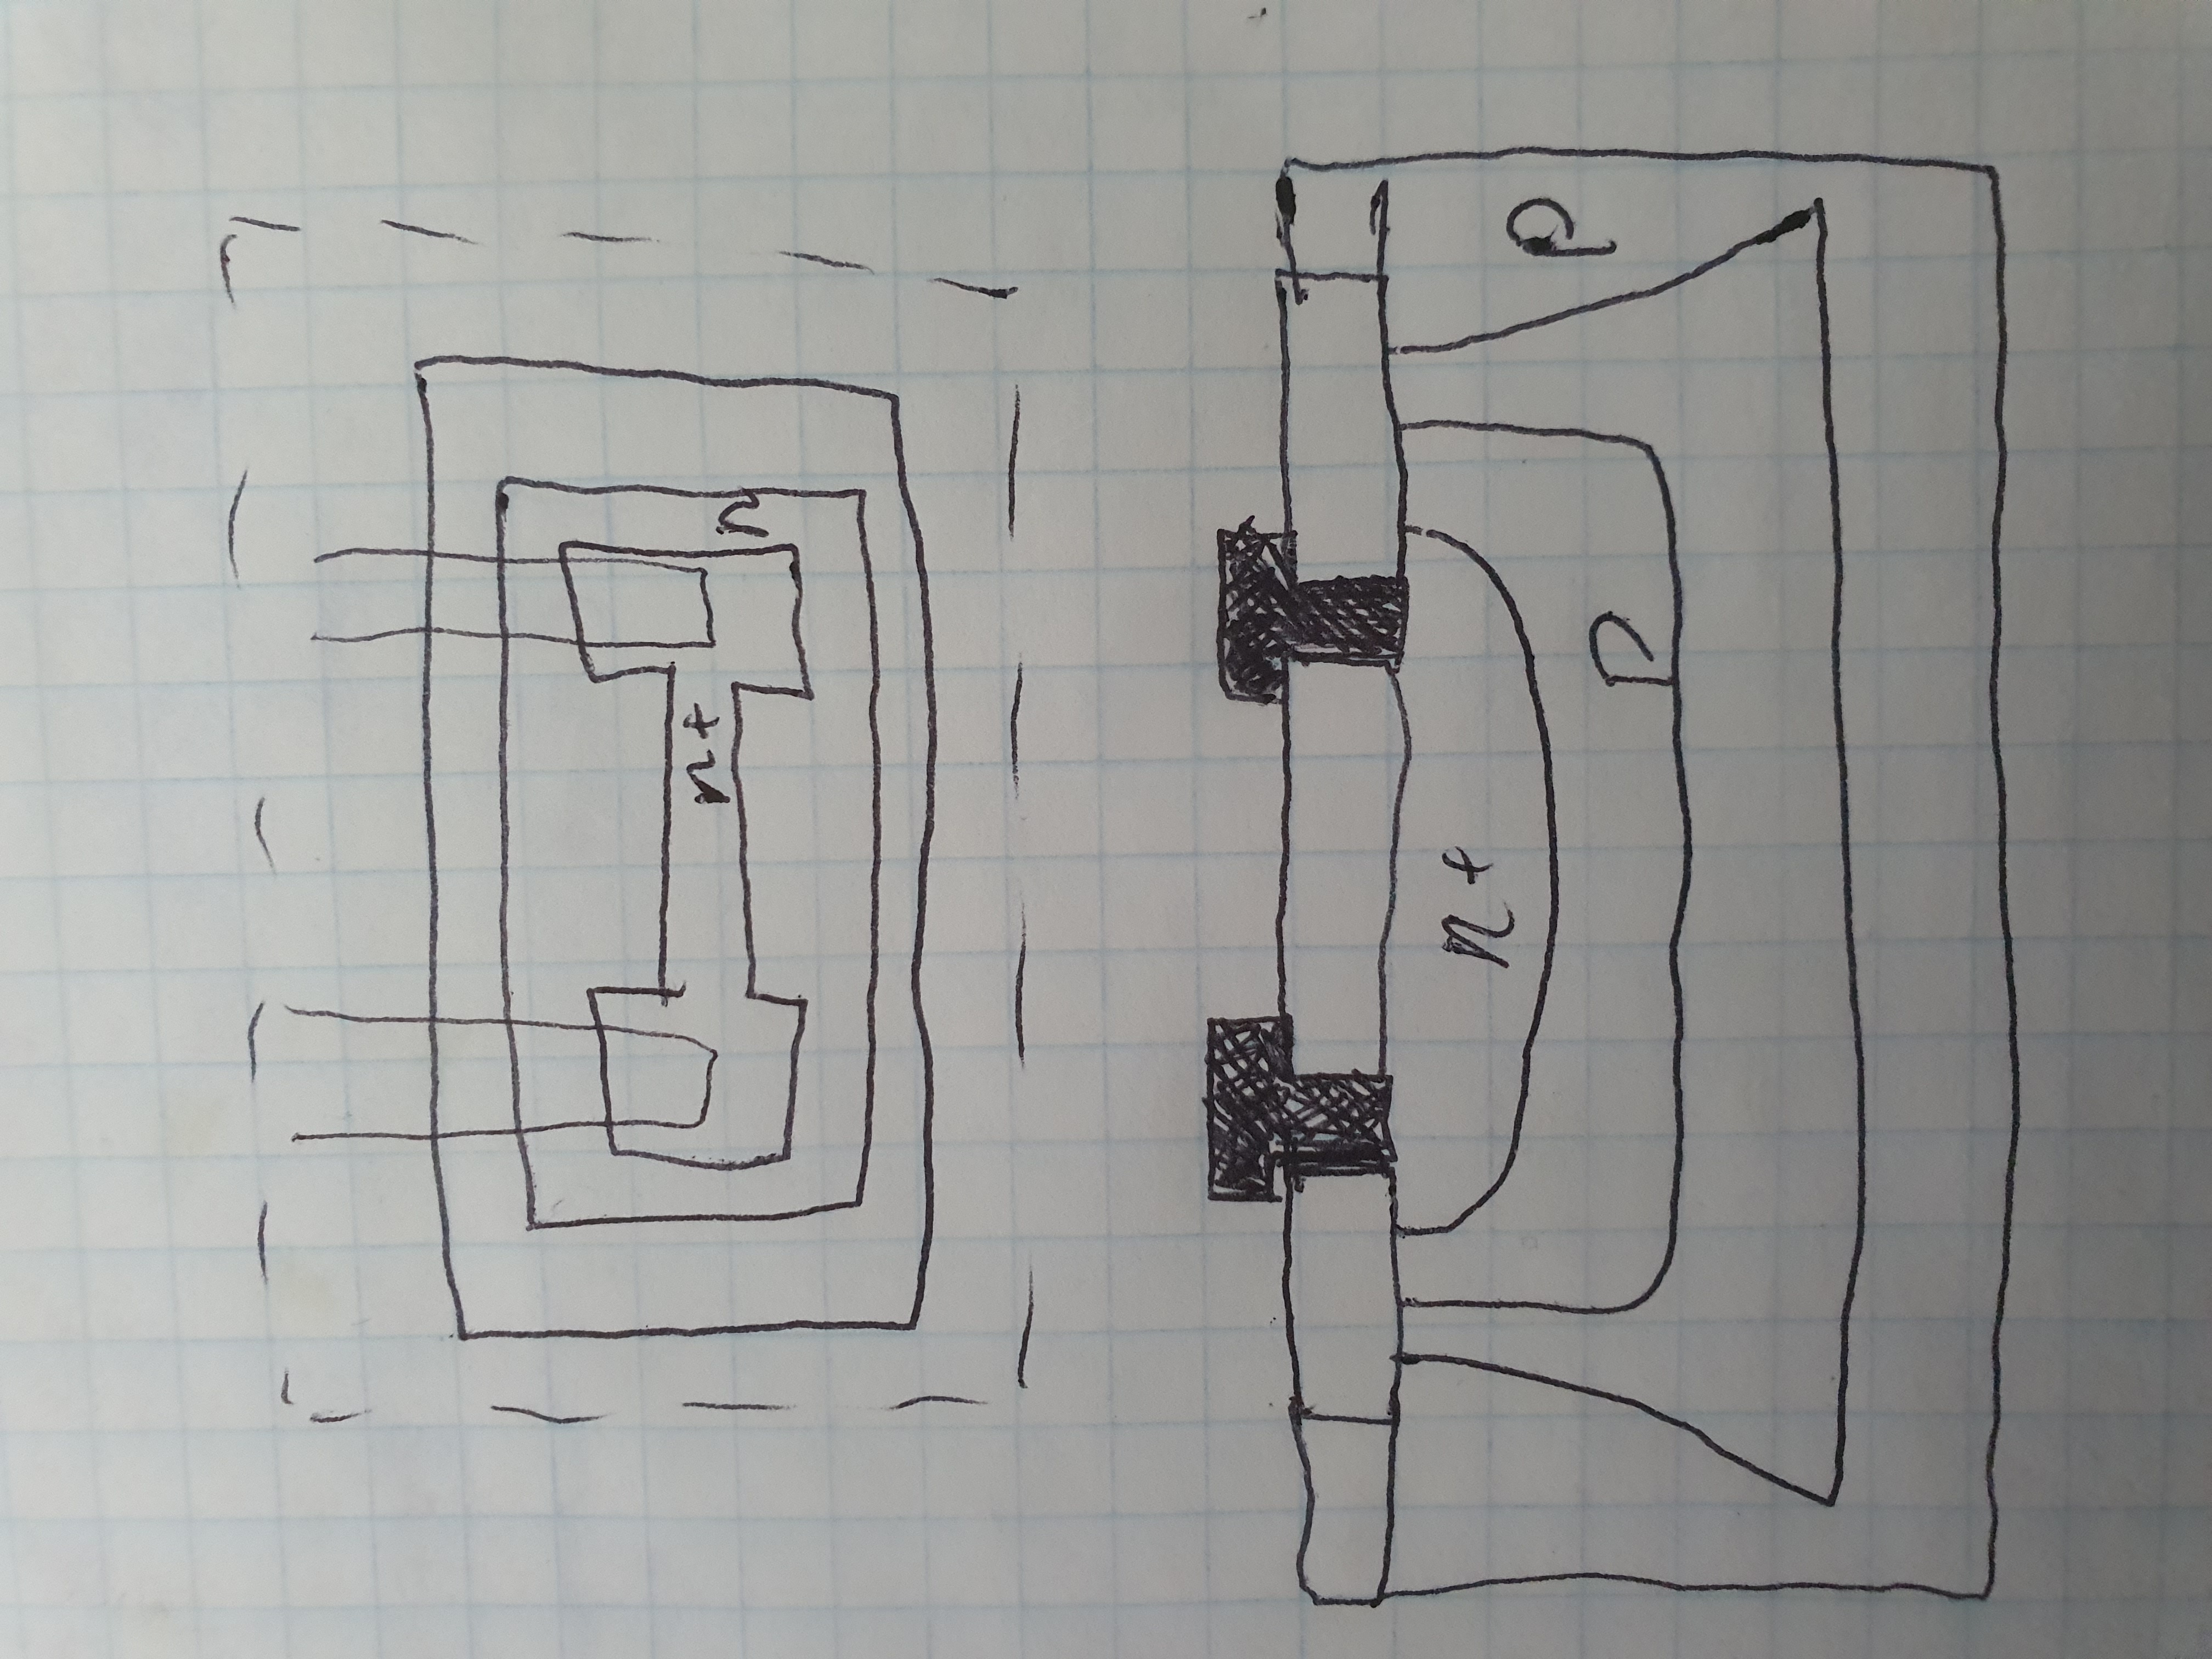
\includegraphics[angle = -90,width=0.4\linewidth]{99.jpg} емітерній області
  \item 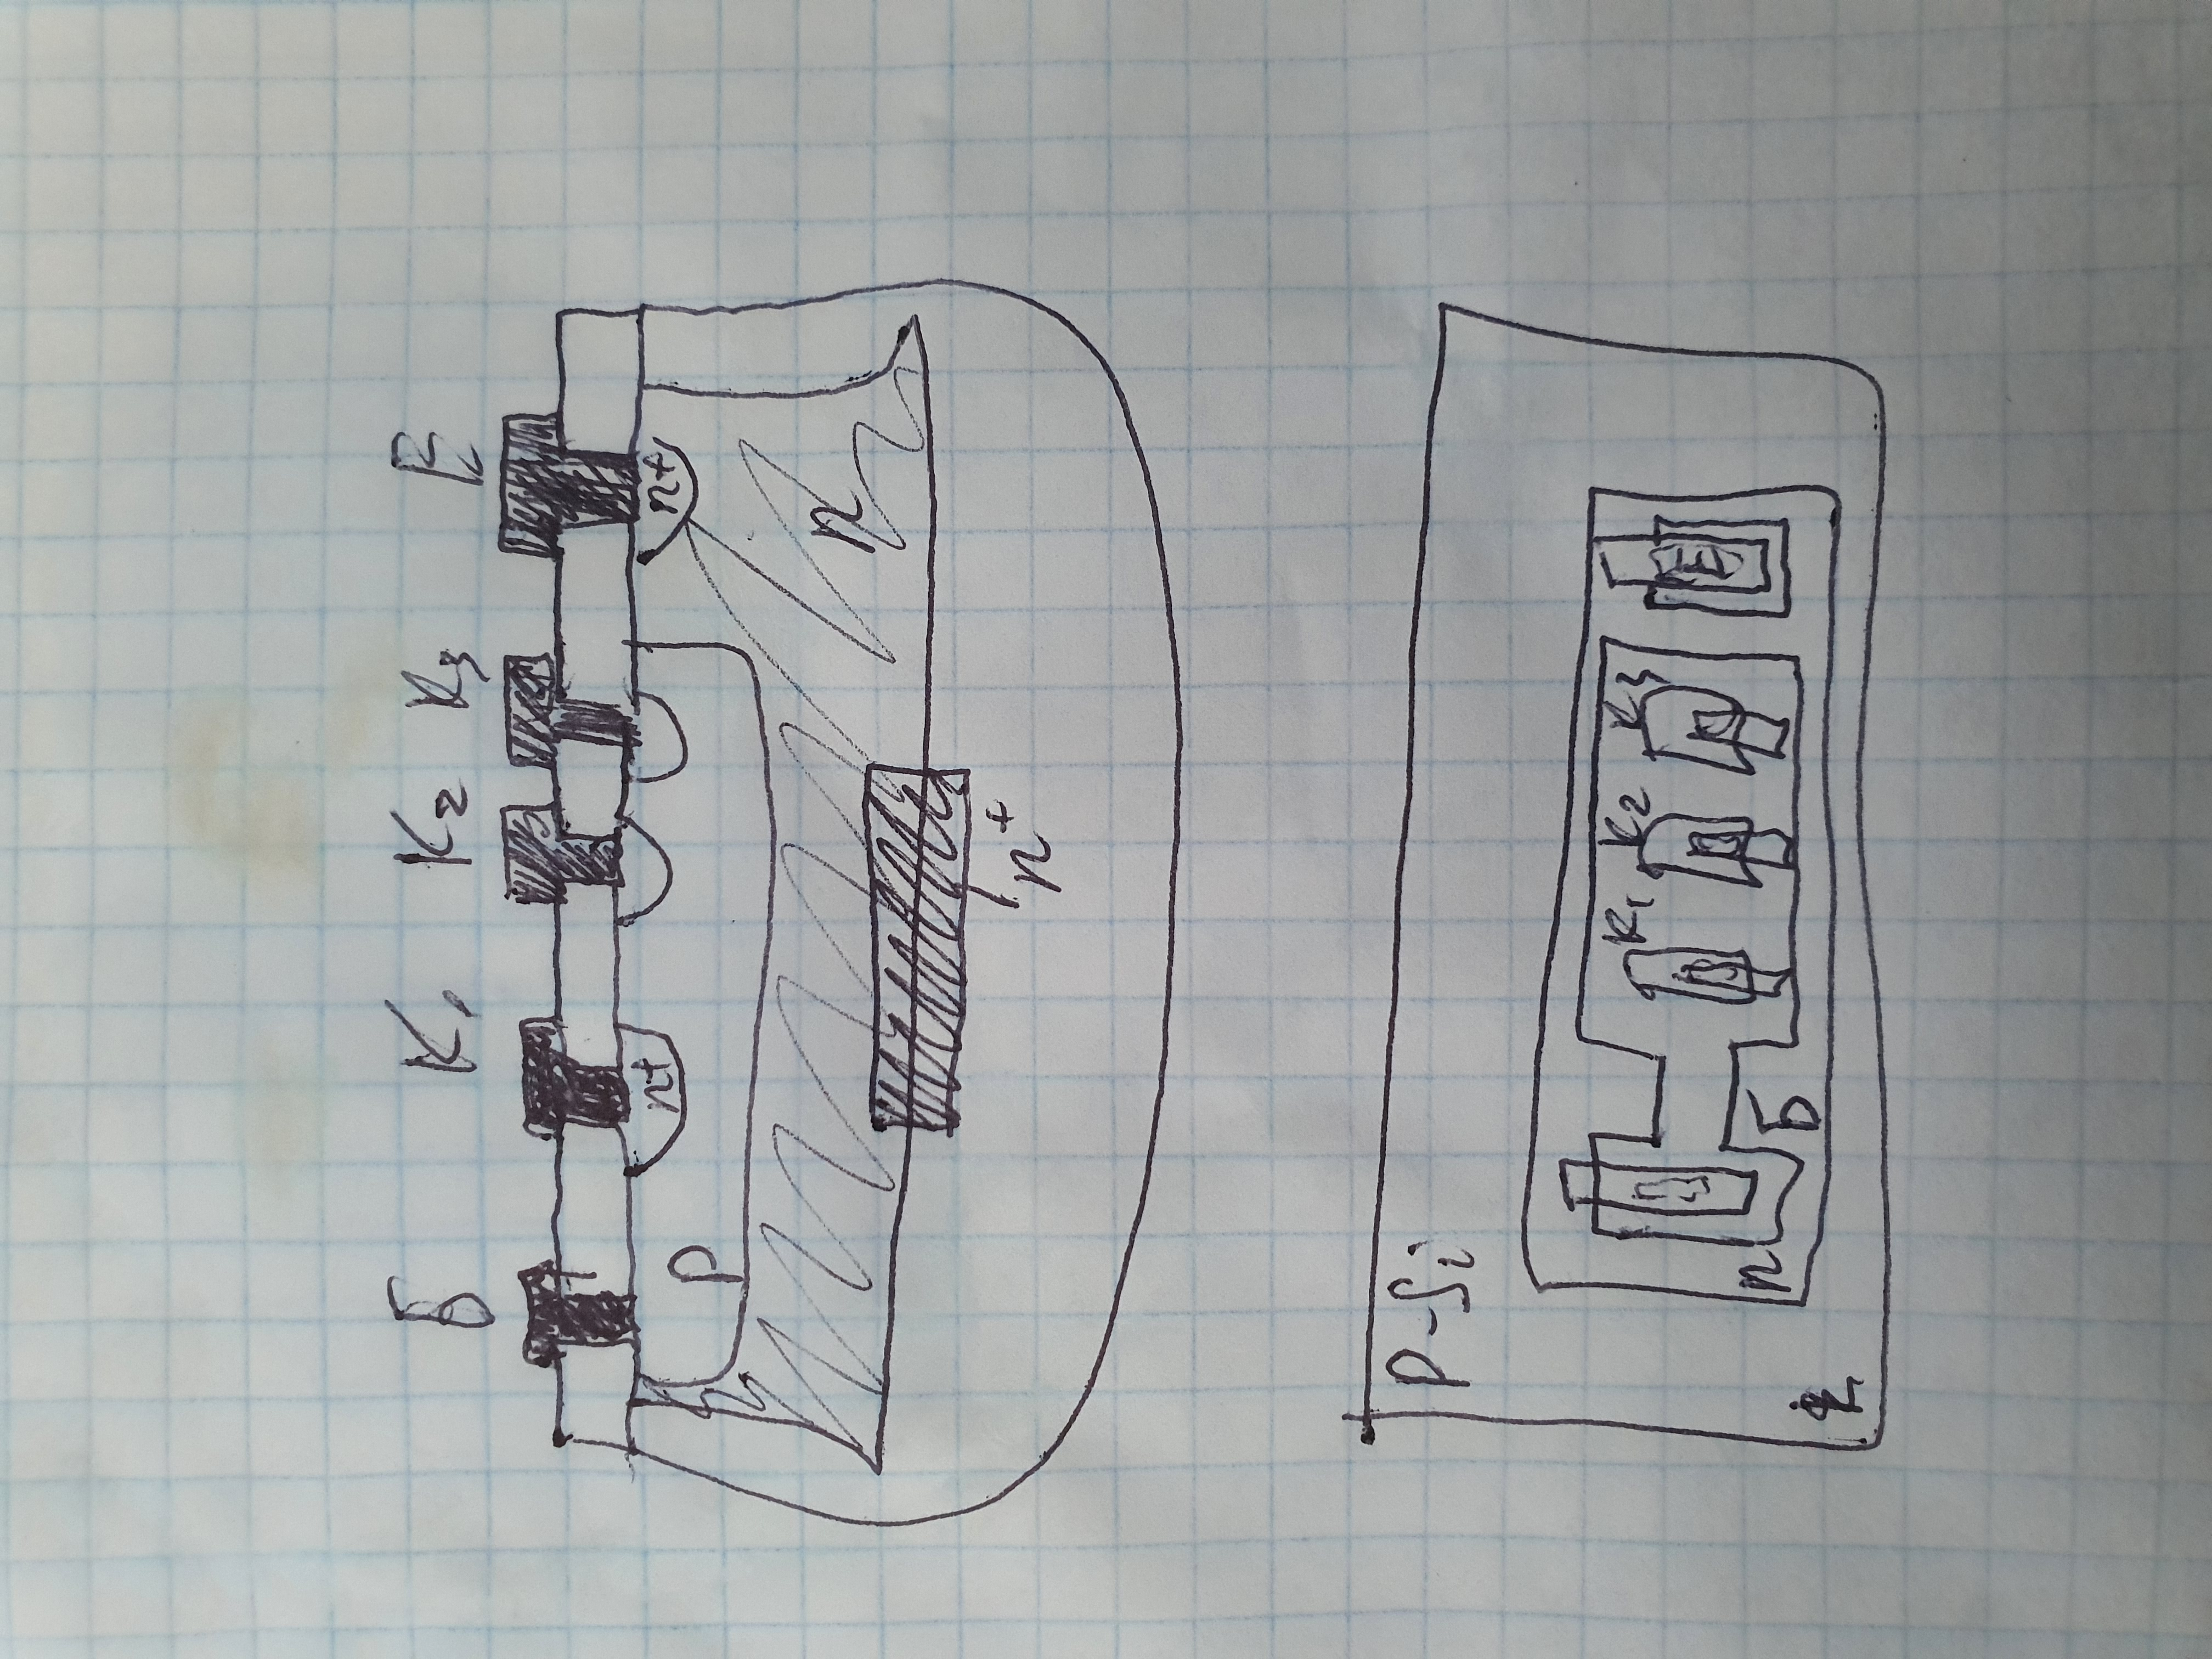
\includegraphics[angle = -90,width=0.4\linewidth]{111.jpg} 
  \item  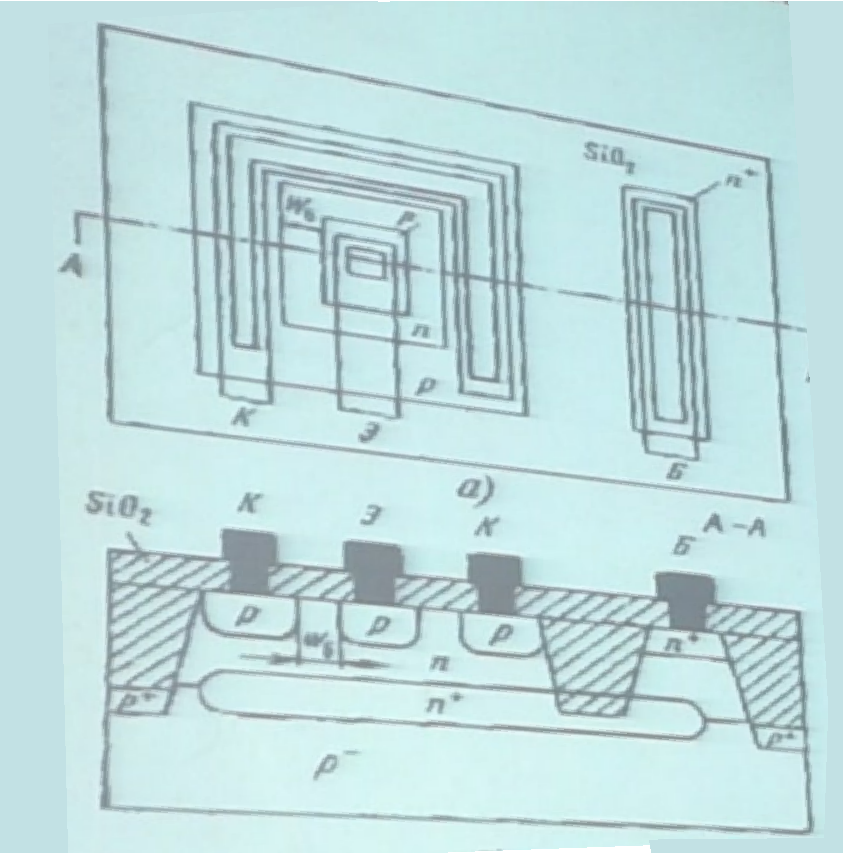
\includegraphics[width=0.4\linewidth]{22.pdf}
  \item






\end{enumerate}




\end{document}
